\section{CP violation sensitivity}
\label{sec:cp_sens}

In this section, various sensitivity results are presented. For the sake of simplicity, unless otherwise stated, only true normal ordering is shown. Possible variations of sensitivity are presented in two ways. Results produced using Asimovs are shown as lines, and differences between two Asimov scenarios are shown with a colored band. Note that the band in the Asimov case is purely to guide the eye, and does not denote a confidence interval. For results produced using many throws of oscillation parameters, systematic and statistical uncertainties, $\sim$300,000 throws were used to calculate the sensitivity for each scenario. The median sensitivity is shown with a solid line, and a transparent filled area indicates the region containing the central 68\% of throws, which can be interpreted as the 1$\sigma$ uncertainty on the sensitivity.

\begin{figure}[htbp]
  \centering
  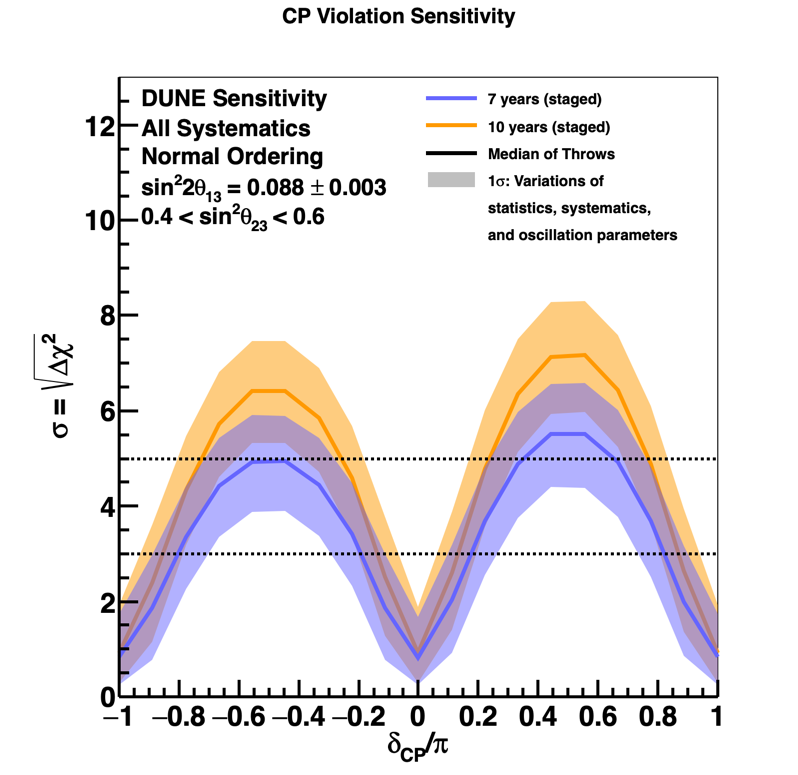
\includegraphics[width=0.98\linewidth, trim={0cm 0cm 0cm 2.3cm}, clip]{cpv_two_exps_throws_nh_2019_v4.png}\\
  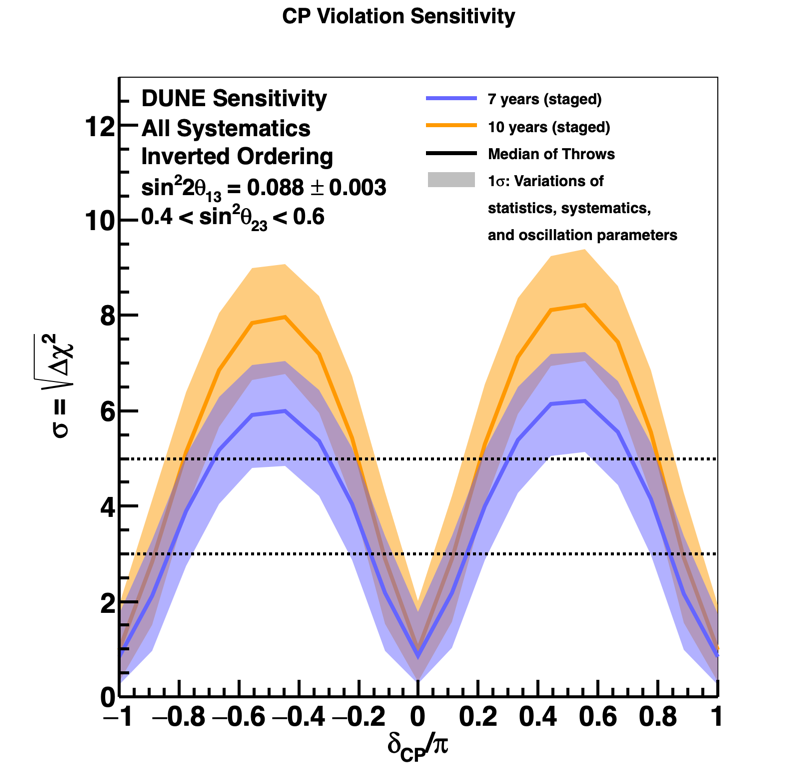
\includegraphics[width=0.98\linewidth, trim={0cm 0cm 0cm 2.3cm}, clip]{cpv_two_exps_throws_ih_2019_v4.png}
  \caption[Significance of the DUNE determination of CP-violation as a function of \deltacp in both \dword{no} and \dword{io}]{Significance of the DUNE determination of CP-violation ($\deltacp \neq [0,\pm\pi]$) as a function of the true value of \deltacp, for seven (blue) and ten (orange) years of exposure, in both normal (top) and inverted (bottom) ordering. The width of the transparent bands cover 68\% of fits in which random throws are used to simulate statistical variations and select true values of the oscillation and systematic uncertainty parameters, constrained by pre-fit uncertainties. The solid lines show the median sensitivity.}
  \label{fig:cpv_nominal}
\end{figure}
Figure~\ref{fig:cpv_nominal} shows the significance with which \dword{cpv} ($\deltacp \neq [0, \pm\pi]$) can be observed in both \dword{no} and \dword{io} as a
function of the true value of \deltacp for exposures corresponding to seven and ten years of data, using the staging scenario described in Section~\ref{sec:rate}, and using the toy throwing method described in Section~\ref{sec:methods} to investigate their effect on the sensitivity.
This sensitivity has a characteristic double peak
structure because the significance of a \dword{cpv} measurement
necessarily decreases around CP-conserving values of \deltacp.
The median \dword{cpv} sensitivity reaches 5$\sigma$ for a small range of values after an exposure of seven years in \dword{no}, and a broad range of values after a ten year exposure. In \dword{io}, \dword{dune} has slightly stronger sensitivity to \dword{cpv}, and reaches 5$\sigma$ for a broad range of values after a seven year exposure.
Note that with statistical and systematic throws, the median sensitivity never reaches exactly zero.


\begin{figure*}[htbp]
  \centering
  \subfloat[24 ktMWyr] {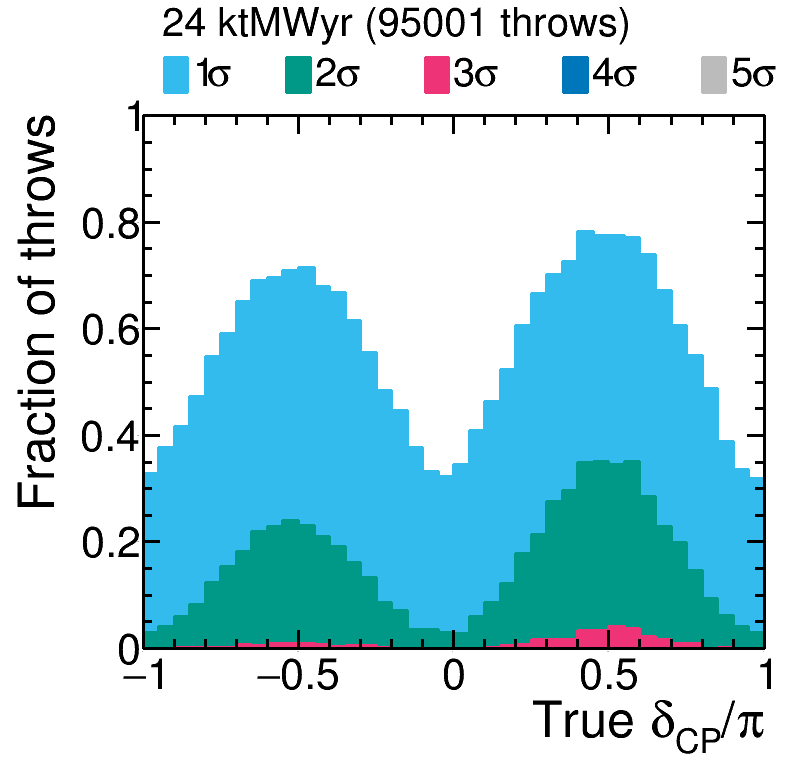
\includegraphics[width=0.33\linewidth]{cpv_throws_24ktMWyr_NH_th13.png}}
  \subfloat[66 ktMWyr] {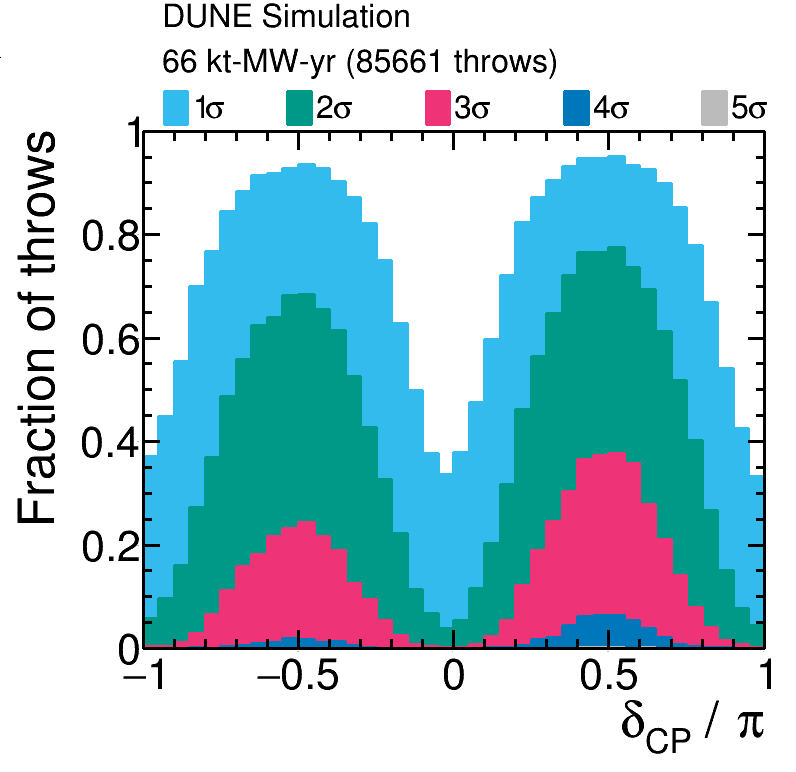
\includegraphics[width=0.33\linewidth]{cpv_throws_66ktMWyr_NH_th13.png}}
  \subfloat[100 ktMWyr]{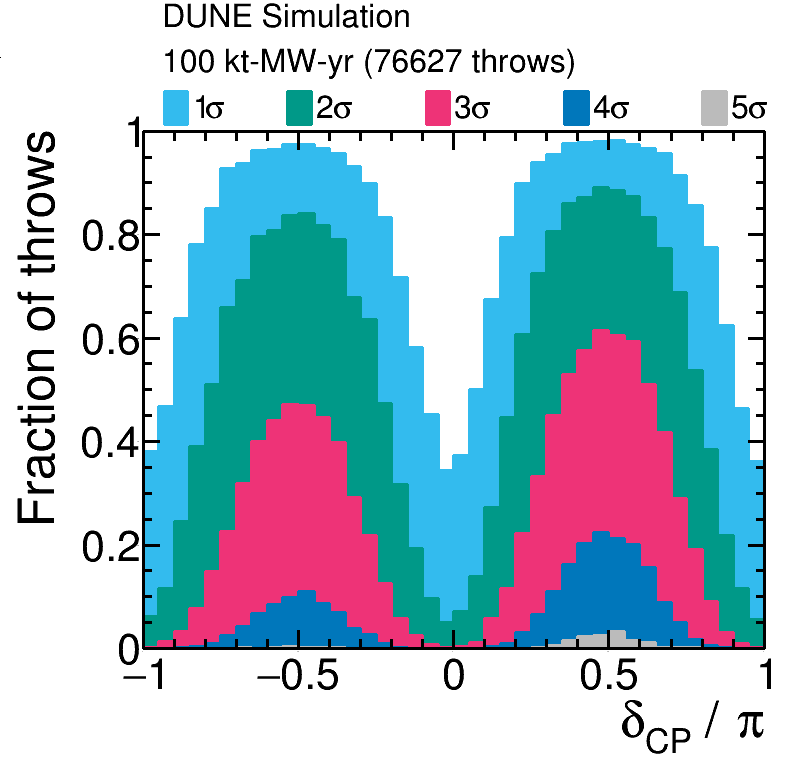
\includegraphics[width=0.33\linewidth]{cpv_throws_100ktMWyr_NH_th13.png}}\\
  \subfloat[150 ktMWyr]{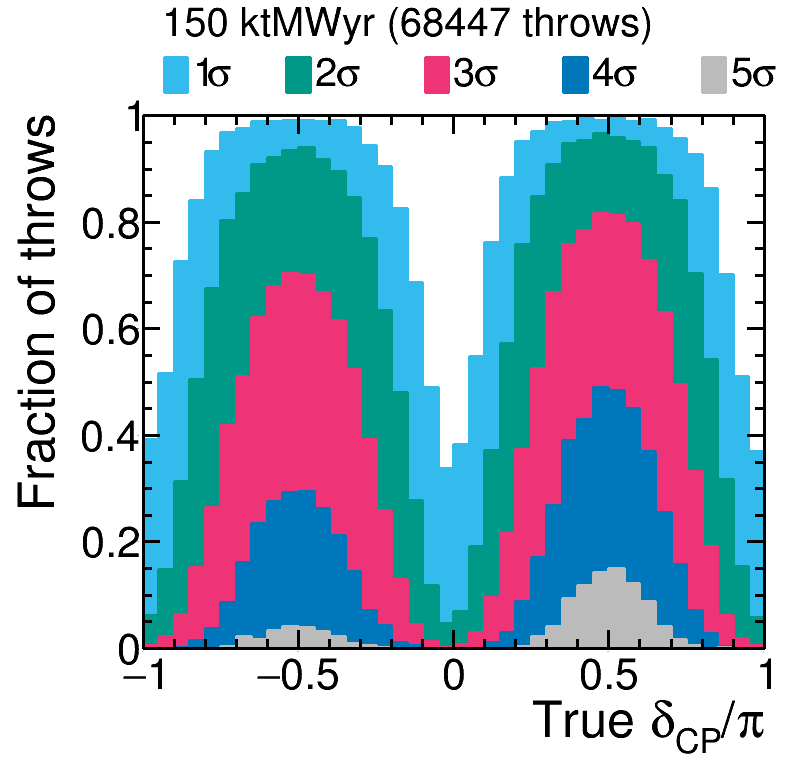
\includegraphics[width=0.33\linewidth]{cpv_throws_150ktMWyr_NH_th13.png}}
  \subfloat[197 ktMWyr]{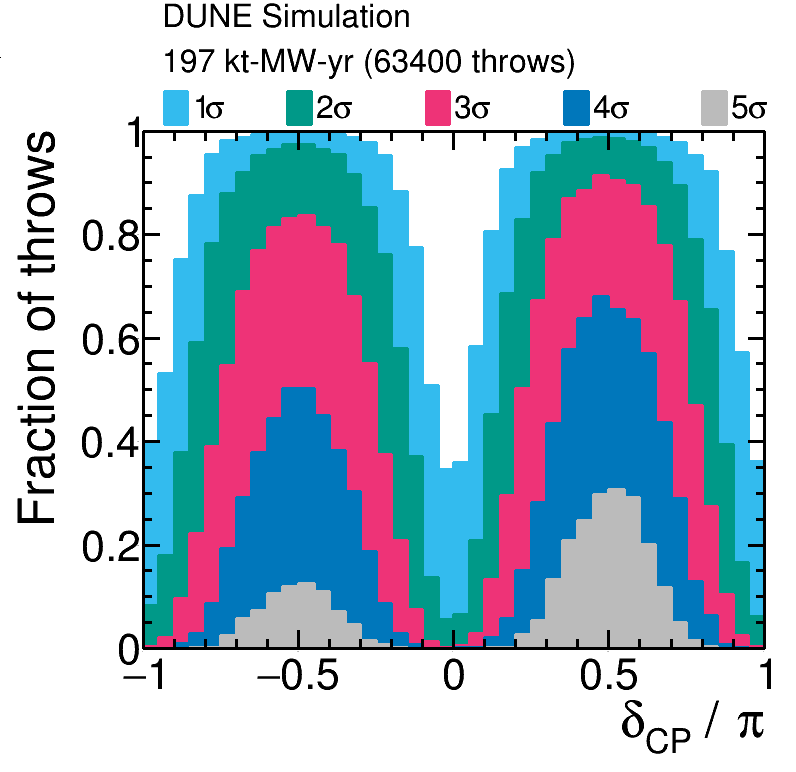
\includegraphics[width=0.33\linewidth]{cpv_throws_197ktMWyr_NH_th13.png}}
  \subfloat[336 ktMWyr]{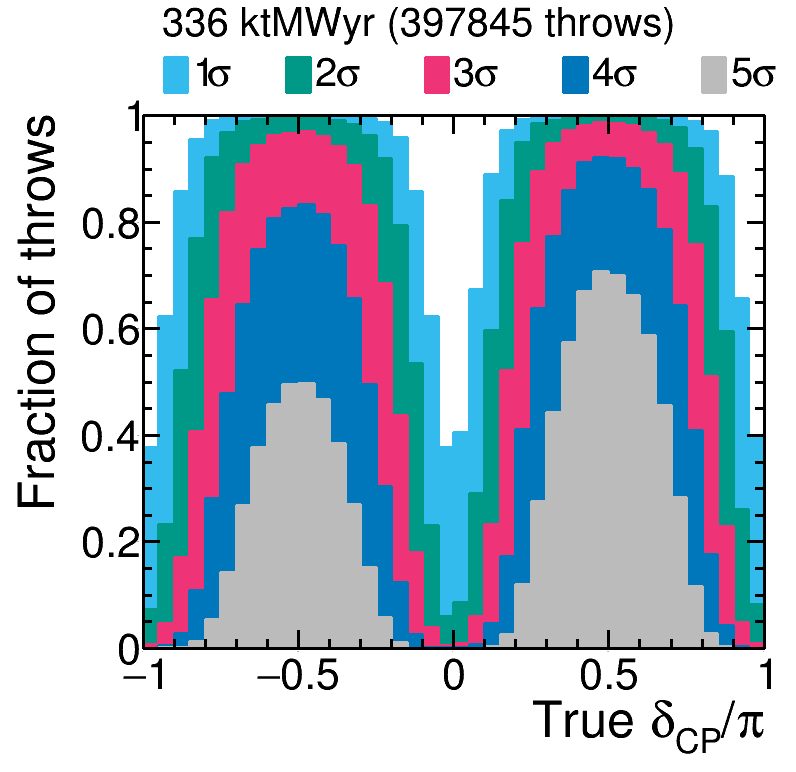
\includegraphics[width=0.33\linewidth]{cpv_throws_336ktMWyr_NH_th13.png}}
  \caption[]{}
  \label{fig:cpv_over_time}
\end{figure*}


\begin{figure}[htbp]
  \centering
  \subfloat[$\deltacp = +\pi/2$] {\includegraphics[width=0.98\columnwidth]{{fraction_throws_vs_exp_dcp0.5}.pdf}}\\
  \subfloat[$\deltacp = -\pi/2$] {\includegraphics[width=0.98\columnwidth]{{fraction_throws_vs_exp_dcp-0.5}.pdf}}
  \caption[]{}
  \label{fig:cpv_vs_exp}
\end{figure}

\subsection{Feldman-Cousins studies}


\begin{figure}[htbp]
  \centering
  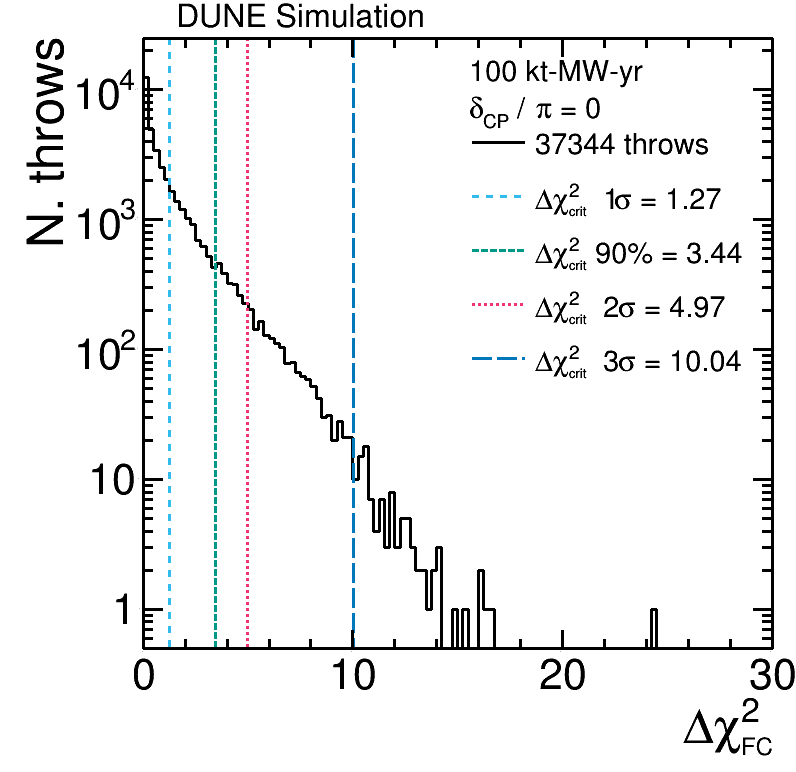
\includegraphics[width=0.98\columnwidth]{nh_FC_ndfd_100ktMWyr_dcp0.png}
  \caption[]{}
  \label{fig:fc_throws}
\end{figure}

\begin{figure}[htbp]
  \centering
  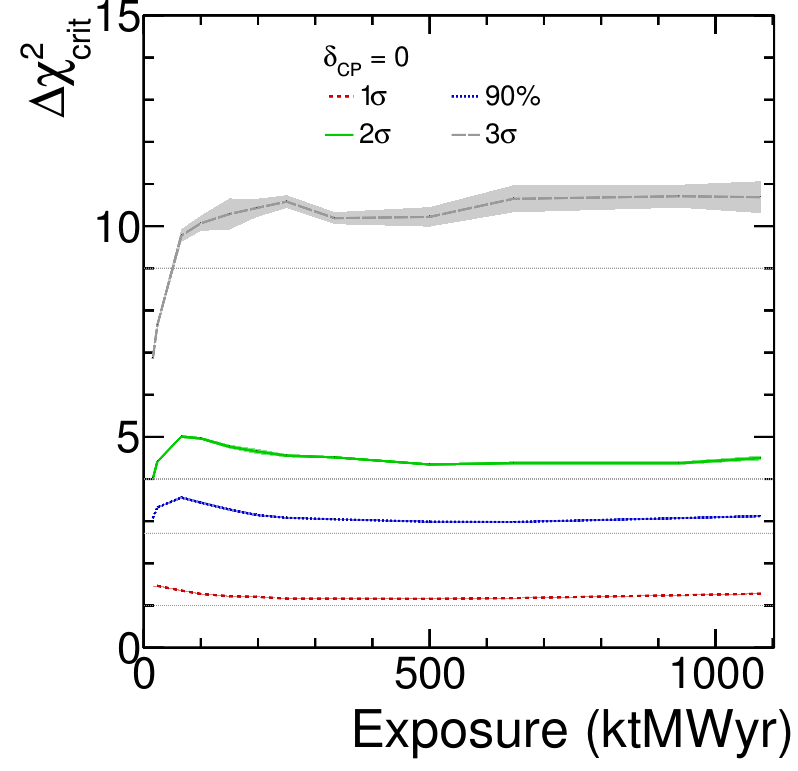
\includegraphics[width=0.98\columnwidth]{dchi2crit_vs_exp_dcp0.png}
  \caption[]{}
  \label{fig:fc_vs_exposure}
\end{figure}

\begin{figure}[htbp]
  \centering
  \subfloat[100 ktMWyr]  {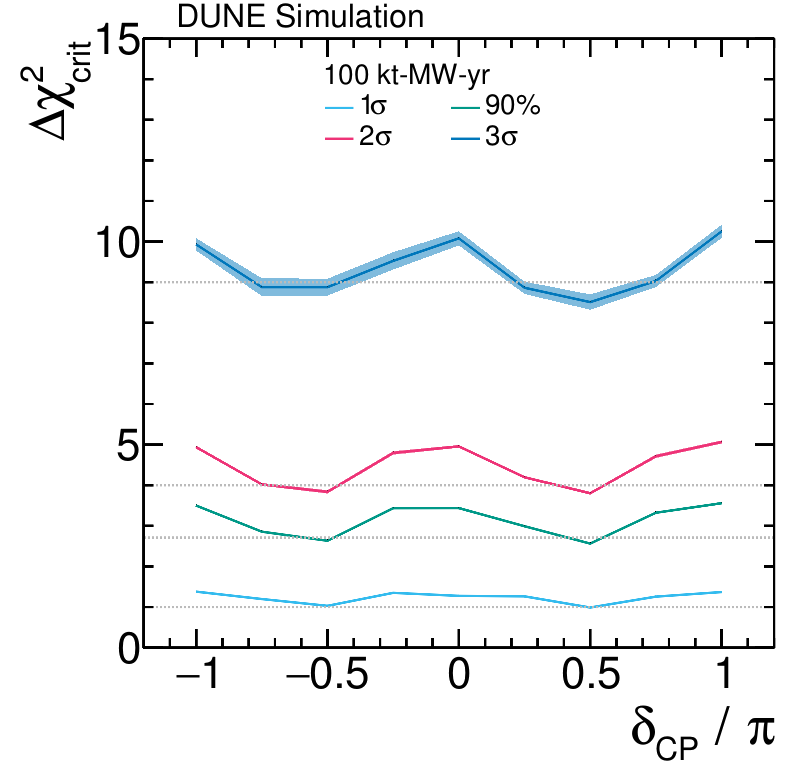
\includegraphics[width=0.98\columnwidth]{dchi2crit_vs_dcp_100ktMWyr.png}}\\
  \subfloat[334 ktMWyr]  {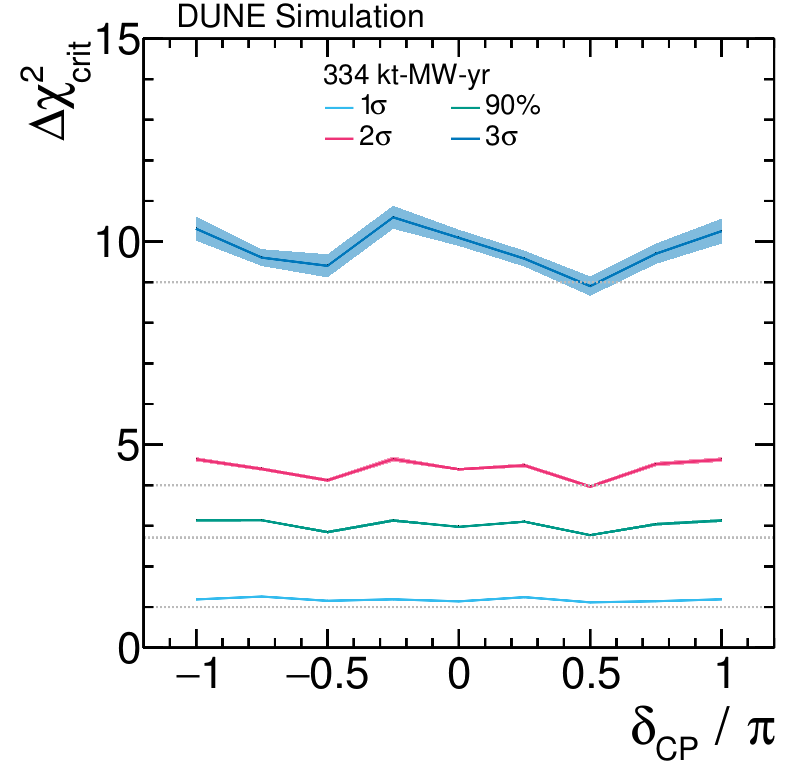
\includegraphics[width=0.98\columnwidth]{dchi2crit_vs_dcp_334ktMWyr.png}}
  \caption[]{}
  \label{fig:fc_vs_dcp}
\end{figure}

\begin{figure*}[htbp]
  \centering
  \subfloat[24 ktMWyr] {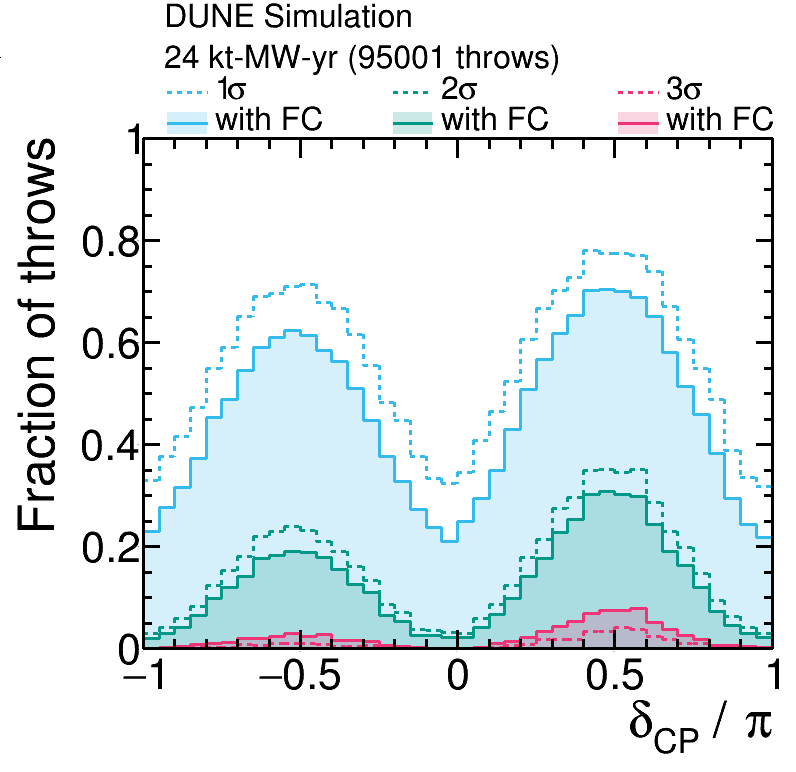
\includegraphics[width=0.33\linewidth]{cpv_throws_withFC_24ktMWyr_NH_th13.png}}
  \subfloat[66 ktMWyr] {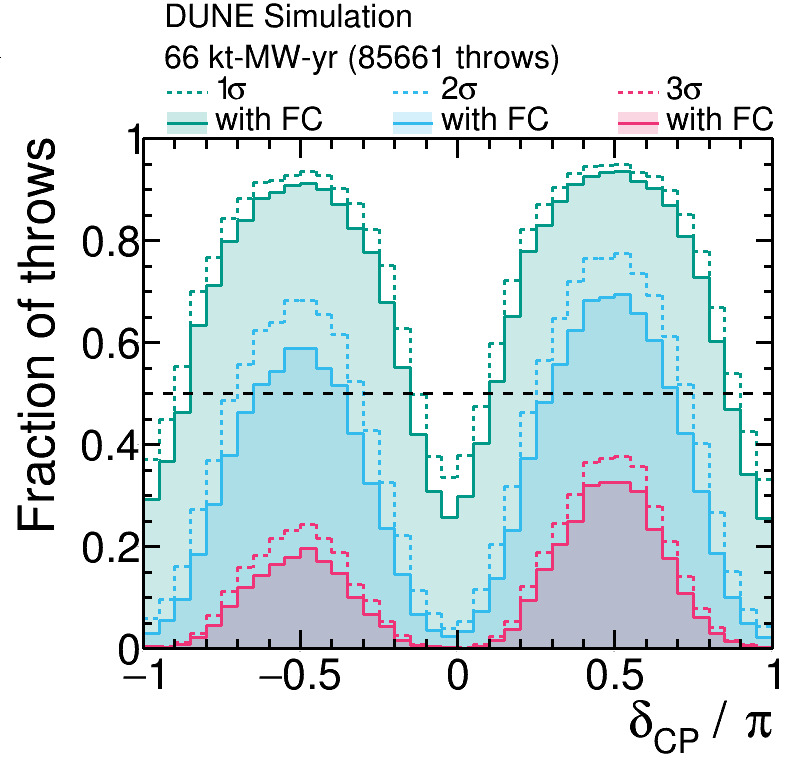
\includegraphics[width=0.33\linewidth]{cpv_throws_withFC_66ktMWyr_NH_th13.png}}
  \subfloat[100 ktMWyr]{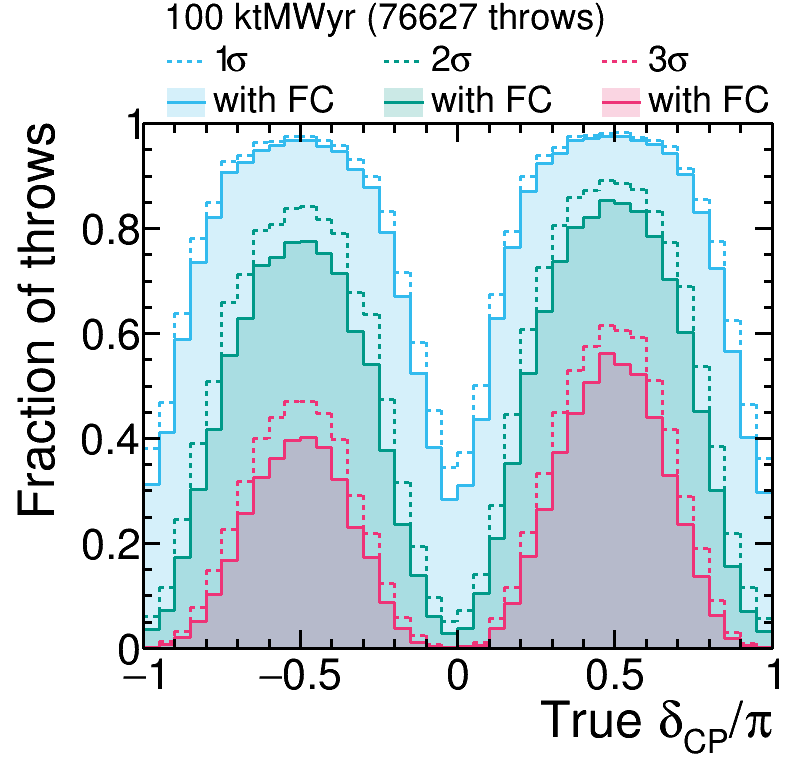
\includegraphics[width=0.33\linewidth]{cpv_throws_withFC_100ktMWyr_NH_th13.png}}\\
  \subfloat[24 ktMWyr] {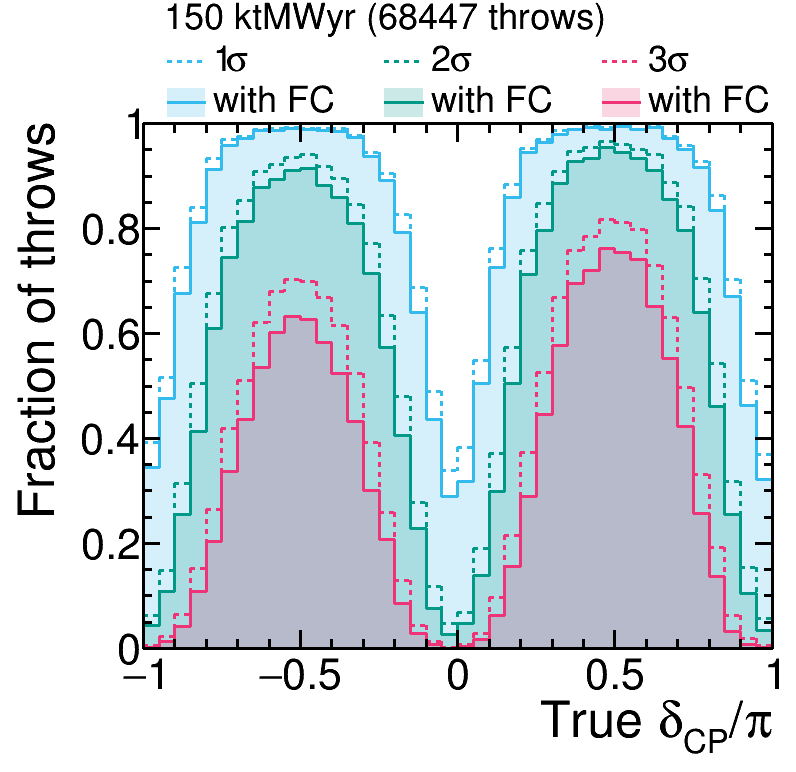
\includegraphics[width=0.33\linewidth]{cpv_throws_withFC_150ktMWyr_NH_th13.png}}
  \subfloat[66 ktMWyr] {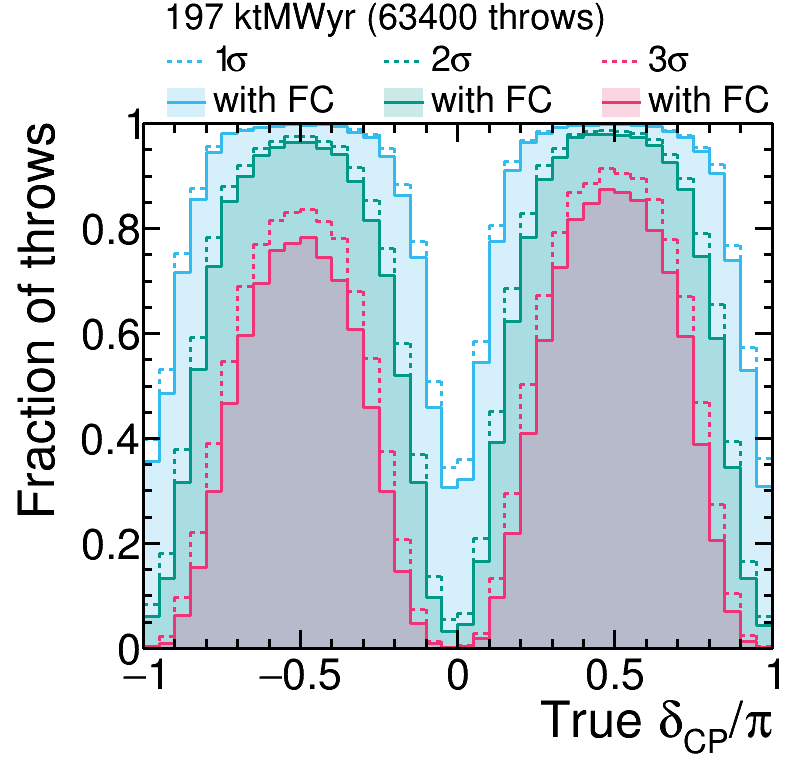
\includegraphics[width=0.33\linewidth]{cpv_throws_withFC_197ktMWyr_NH_th13.png}}
  \subfloat[100 ktMWyr]{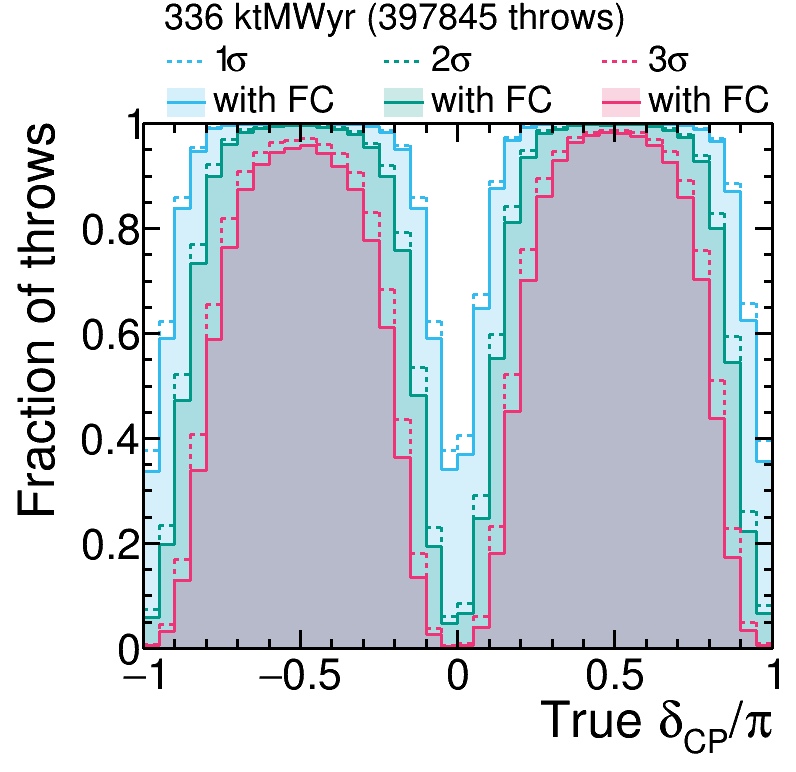
\includegraphics[width=0.33\linewidth]{cpv_throws_withFC_336ktMWyr_NH_th13.png}}
  \caption[]{}
  \label{fig:cpv_over_time_fc}
\end{figure*}

\begin{figure}[htbp]
  \centering
  \subfloat[$\deltacp = +\pi/2$] {\includegraphics[width=0.98\columnwidth]{{fraction_throws_vs_exp_dcp0.5_FC}.pdf}}\\
  \subfloat[$\deltacp = -\pi/2$] {\includegraphics[width=0.98\columnwidth]{{fraction_throws_vs_exp_dcp-0.5_FC}.pdf}}
  \caption[]{}
  \label{fig:cpv_vs_exp_fc}
\end{figure}

\FloatBarrier
